\documentclass[14pt,fleqn]{extarticle}
\RequirePackage{prepwell}

\previewoff 

\begin{document} 
\begin{snippet}
    \correct
    
    The shaded portion is the area bound by $y=x^2, x = 1$ and 
    the \xaxis
    
    \begin{center}
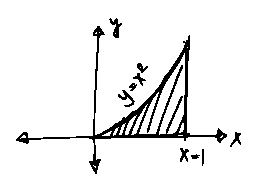
\includegraphics[scale=1.4]{figure.eps}
\end{center}

When this area is rotated around the \xaxis, then the volume 
of the resulting solid is 
\[ \qquad V = \int_0^1 \pi x^4\cdot dx = \frac{\pi}{5} \]
    
    \reason
    
    Imagine a thin strip $AB$ of width $dx$ at some $x$ -- as shown below 
    \begin{center}
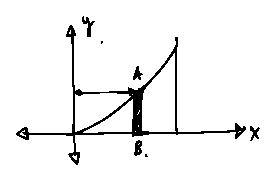
\includegraphics[scale=1.4]{diagram.eps}
\end{center}
 
When $AB$ is rotated around the \xaxis, then one gets the following cylinder 
\begin{center}
  \begin{tabular}{lNNN}
   \toprule
        &  \text{Radius} & \text{Height} & \text{Volume } (dV) \\
   \midrule 
   Cylinder & y = x^2 & dx & \left(\pi y^2 \right)\cdot dx = \pi x^4\cdot dx \\
    \bottomrule
  \end{tabular}
\end{center}

Add up the volume of all such cylinders to get the volume of the generated solid  

\begin{align}
	V &= \int_0^1 dV = \int_0^1 \pi x^4\cdot dx \\
	&= \pi \left[\frac{x^5}{5} \right]_0^1 = \frac\pi{5} 
\end{align}
\end{snippet} 
\end{document} 